\chapter{Platinenaufbau}
\label{sec:Platinenaufbau}
\pagestyle{scrheadings}

\section{Vorüberlegungen} 
Die Zielsetzung im Aufbau der Platine war eine kompakte Basisstation mit sechs Transceivern und einer zentralen Steuereinheit. Um sicherzustellen, dass alle Antennen gleichmäßig in die sechs vorgegebenen Raumrichtungen abstrahlen, sollte bereits die Platine symmetrisch aufgebaut werden. Dazu wurde zuerst das Layout der sechs identischen Transceiver-Einheiten mit dem TDA5340 Baustein und den Antennenanschlüssen erstellt und anschließend gleichmäßig um die weiteren für die Schaltung notwendigen funktionellen Segmente angeordnet.

 
\section{Layoutprogramm Altium Designer}
Bei dem Entwicklungswerkzeug \enquote{Altium Designer} des Entwicklers Altium Limited handelt es sich um ein System zum Entwurf von  gedruckten  Schaltungen oder \acp{PCB}. Ein solches Programm wird auch als \ac{EDA} oder ECAD für electronic \ac{CAD} bezeichnet, da es den Entwickler bei der Umsetzung der Anforderungen in einen Schaltplan und später eine Platine unterstützen soll.
Wie viele andere \ac{EDA}-Programme ist auch Altium Designer so aufgebaut, dass sich der Entwickler zuerst mit dem allgemeinen symbolisierten Schaltplan befassen kann und erst zu einem späteren Zeitpunkt die tatsächliche Anordnung der Bauteile auf dem \ac{PCB}-Substrat festgelegt wird. Somit können zuerst im Schematic Editor die Funktionen der Schaltung umgesetzt werden. Dazu werden die verwendeten Bauteile aus zuvor angelegten Bibliotheken verwendet oder es werden bestehende Libraries genutzt, die etwa vom Hersteller der Bauteile zur Verfügung gestellt werden. Altium selbst bietet hierfür auch diverse Möglichkeiten an und stellt Bauteile nach Hersteller und Art geordnet bereit.
In den Bibliotheken sind alle im weiteren Verlauf benötigten Informationen über die einzelnen Bauteile enthalten. So liegen dort etwa  entsprechenden Abbildungen für das Bauteil im  Schaltplan  vor. In den so genannten \enquote{Footprints} zu jedem Bauteil, welche ebenfalls in den Bibliotheken enthalten sind, wurde zuvor die, für das physikalische Gehäuse, notwendigen Abmessungen, Lötpads und Ausmaße für Lötstopplack um das Bauteil festgelegt. Da es Bauteile, wie den verwendeten  Mikrocontroller, in verschiedenen Gehäusen geben kann, besteht somit auch die Möglichkeit hier zwischen verschiedenen Footprints zu wählen. Da viele Gehäuse herstellerübergreifend genormt sind, konnten teilweise bestehende Footprints genutzt  oder diese mehrfach verwendet werden.



Wie bereits erwähnt wird im \ac{EDA}-Programm zuerst der symbolische Schaltplan erstellt. Dieser wird anschließend in ein Layout für eine Platine umgewandelt. Die zu den Schaltplansymbolen korrespondierenden Footprints werden dazu auf dem Layout der Platine angeordnet und durch das \enquote{Routing} werden die Leiterbahnen definiert.
Altium Designer ist dabei in drei Teilbereiche unterteilt: im \enquote{Board Planning Mode}  liegt der Fokus auf dem Anordnen der einzelnen Bauteile und Komponenten auf der Leiterplatte, außerdem wird in diesem Bereich die Form und das Ausmaß der Leiterplatte festgelegt. Im 2D-Modus des \ac{PCB}-Editor lassen sich anschließend die aus der Definition im Schaltplan ergebenden elektrischen Verbindungen örtlich auf den verschiedenen Kupferebenen (Layern) anordnen. Die Hauptarbeit findet also in diesem Teil des \ac{PCB}-Editors statt. Der 3D-Modus dient anschließend zur Evaluation des Designs und zur Anpassung an Gehäuse oder andere Komponenten.
In den verschiedenen Ebenen oder \enquote{Layern} sind die Kupferebenen und andere Schichten der späteren Platine wie der Bestückungsdruck oder der Lötstopplack gesammelt. Jede Ebene entspricht daher einer zu fertigenden Schicht und existiert für die Vorder- und Rückseite der Platine. Beim Bewegen eines Bauteils wird nicht nur die markierte Abmessung, sondern etwa auch die Anschluss-Pads und der Lötstopplack auf denen entsprechenden Ebenen bewegt. Durch Vias sind elektrische Verbindungen zwischen den Kupferschichten möglich.

Für die Basisstation wurden zwei Kupferebenen und ausschließlich sogenannte \ac{SMD}-Bauelemente verwendet. Diese liegen nur auf der Oberfläche der Platine auf und sind durch ihre Lötverbindungen befestigt. Die Vorteile dieser Bauteile sind der geringe Preis und die kleinen Abmessungen. 

%Ebenfalls...    Layers/ebene, top, bot, bestückungsdruck, solderresin
%lagenanzahl 
%lötpad
%platinenmaterial (zb bezüglich wärmemangement)s. Übung LEKFZ
%welche Bauteile in eigener Lib?
%verwendung SMD Bauteile

%Bauteileingabe und schaltplan
%Multi channel - multi sheet
Wegen der Größe des Projekts wurde zur besseren Übersicht ein  so genanntes \enquote{Multi-Sheet-Design} erstellt. Dadurch war es möglich, die verschiedenen funktionellen Blöcke der Basistation auf getrennte Blätter des Schaltplans zu verteilen. Der Mikrocontroller, die Spannungsversorgung und der Transceiver, sowie die für eine Netzwerkkommunikation notwendigen Bauteile  wurden dabei auf unabhängigen Seiten angeordnet und dort die elektrischen Verbindungen erstellt.

Da der Transceiver und die entsprechende Peripherie sechsmal in identischer Anordnung und Beschaltung verwendet wurden und auch auf dem \ac{PCB}-Substrat mehrfach mit Leiterbahnen verbunden und angeordnet werden mussten, wurde hierfür ein so genanntes \enquote{Multi-Channel}-Design gewählt. In Altium Designer können mit diesem Feature identische Schaltungsteile einmal angeordnet, mit Leiterbahnen verbunden  und dieses Design auf alle anderen entsprechenden Schaltungsteile angewendet werden. Somit muss das aufwändige Anordnen der Bauteile und die Führung der Leiterbahnen nur bei einem der Kanäle durchgeführt werden.  Dazu wurde mit Hilfe eines übergeordneten Sheet-Symbols der Schaltplan des Transceivers in den Schaltplan des Mikrocontrollers eingefügt und diesem somit untergeordnet. Über Ports, welche zum  Schaltplansymbol hinzugefügt werden, lassen sich elektrische Verbindungen zwischen Netzen innerhalb der Schaltpläne für Transceiver  und Mikrocontroller erstellen. Dabei wird im Transceiver-Schaltplan ein Port hinzugefügt, der mit dem gewünschten elektrischen Netz  verbunden werden kann. Auf dem Schaltplansymbol im Mikrocontroller-Schaltplan wird ein entsprechender gleichnamiger Port erstellt, der mit Netzen am Mikrocontroller verbunden werden kann. Da die drei Verbindungen der \ac{SPI}-Kommunikation jeweils aus einem Netz bestehen und etwa alle \acs{MISO}-Leitungen an demselben Pin des XMC4500 und denselben Anschluss bei allen TDAs angebunden sind, konnte hierfür ein einfacher Port verwendet werden. Alle anderen Anschlüsse, wie etwa die Auswahlleitung für die \ac{SPI}-Verbindung, welche für jede der sechs verschiedenen Transceiver-Einheiten mit einen anderen Anschluss des Mikrocontrollers verbunden sein mussten, wurden deswegen mit dem Repeat-Kommando erstellt. So wird im untergeordneten Schaltplan, in diesem Fall dem des TDA, der Port beliebig benannt, etwa als \enquote{NCS}. Der auf dem Schaltplansymbol erstellte korrespondierende Port wird dagegen in \enquote{Repeat(NCS)} umbenannt. Eine Verbindung mit dem Port auf dem Schaltplansymbol wird dadurch zu einem Bus. Dieser kann aufgetrennt werden und die Verbindungen von jedem Kanal als einzelnen Signal an den Mikrocontroller angeschlossen werden. Globale Netze wie die Versorgungsspannung von \unit[3,3]{Volt} oder die Masse müssen dabei nicht als Port hinzugefügt werden. Altium Designer stellt deren Verbindungen automatisch her. Wird nun noch der Name des Schaltplansymbols nach dem folgenden Muster angepasst, wird Altium Designer beim Kompilieren des Projektes ein Multi-Channel-Design erstellen, die Kanäle wie angegeben durchnummerieren und den Kanal im \ac{PCB}-Editor entsprechend mehrfach erstellen. Dazu sollte der Name die Struktur \enquote{Repeat(<Name>,<Startnummer> ,<Endnummer>)} aufweisen. Anschließend kann die Anordnung und das Routing des ersten Kanals erfolgen. Da für jeden Kanal ein eigener so genannter \enquote{Room} erstellt wird, lassen sich, nach dem Erstellen der Leiterbahnen des ersten Kanals, die Anordnungen der Bauteile und Leiterbahnen mit dem \enquote{Copy Room Format}-Befehl auf alle anderen Kanäle erweitern. Ein Room bezeichnet dabei eine Gruppe an Elementen im PCB-Editor und einen Bereich der Platine, in dem diese angeordnet sind und erlaubt so das Verschieben ganzer Schaltungsteile auf der Platine. Der Schaltplan des Hauptkanals, welcher einen einzelnen der sechs Kanal darstellt, ist in Abbildung \ref{fig:schemTDA} zu erkennen.


% Bestückungsdruck
Altium Designer nummeriert automatisch die verwendeten  Bauelemente durch, um die genaue Identifikation eines Bauteiles zu erlauben und erstellt automatisch einen Aufdruck neben dem Lötpad mit dem Bauteilnamen in der entsprechenden Ebene. Ein solcher Bestückungsdruck zur leichteren Anordnung der Bauteile auf der fertig entwickelten Platine wurde nur auf der Hauptplatine erstellt. Auf den Teilplatinen für die Transceiver wurde dieser aus Platzgründen weggelassen.

% Design Rule Check
Um sicherzustellen, dass die sich aus der Bauteilanordnung ergebenden Pads und die Leiterbahnen auch fertigbar sind, stellt Altium Designer zwei \acp{DRC}  bereit. Im ersten Live-\ac{DRC} werden \enquote{Violations}, also Bauteile mit Verstößen gegen die Designregeln, durch ein farbiges Overlay markiert. Im folgenden kompletten Test zeigt Altium alle weiteren Verstöße an. Als Verstoß gelten etwa Leiterbahnen unterschiedlicher Netze, die sich berühren und zu einem Kurzschluss führen würden oder auch  Verletzungen der festgelegten Abstandsregeln (Clearance). Alle Regeln für Violations können im \enquote{PCB Rules Editor} eingestellt werden und so an die Möglichkeiten des \ac{PCB}-Herstellers angepasst werden. Da die Leiterplatte für die Basisstation von Multi Circuit Boards Ltd. hergestellt wurde, konnten die auf der Webseite dieses Herstellers angegebenen Designregeln für den \ac{DRC} übernommen werden.
Da Altium Designer im \ac{DRC} sich kurzgeschlossene und falsch verbundene Pads angezeigt werden, muss kein extra \enquote{Layout vs. Schematic}-Test durchgeführt werden, der den vorher erstellten Schaltplan mit dem Layout abgleicht. Solche Unterschiede zwischen Schaltplan und dem \ac{PCB}-Layout würden durch den \ac{DRC} bereits angezeigt.

\section{Verwendete Hardware}

\subsection{TDA5340}
Der verwendete Transceiver TDA5340 wird von Infineon Technologies AG  entwickelt und vertrieben. Er ist Teil der SmartLEWIS Produktfamilie die  energiesparende Lösungen für Funkanwendungen im Frequenzspektrum unterhalb von einem Gigahertz bietet. 
Der Transceiver kommuniziert mit seinem Host über das \ac{SPI}-Protokoll, der Mikrocontroller ist in diesem Fall sternförmig mit den einzelnen TDA-Bausteinen verbunden, die als Slaves fungieren. Die Daten werden mit drei gemeinsamen Leitungen übertragen, eine vierte Leitung dient dem XMC zur Auswahl des gewünschten Slaves für die Kommunikation. Diese \ac{NCS}-Leitung arbeitet active-low, sodass der jeweilige TDA5340 eine Interaktion akzeptiert, sobald diese vom XMC-Baustein auf Massepotential gezogen wird. Von den drei eigentlichen Datenleitungen fungiert eine als reiner Ausgang des Masters bzw. Dateneingang des TDA (\acs{MOSI}), eine zweite als Eingang des Masters (\acs{MISO}) und die dritte als ein vom Mikrocontroller getriebenes Clock-Signal. Bei dem auf \acs{MISO} und \acs{MOSI} anliegenden Signal handelt es sich um ein unipolar kodiertes non-return-to-zero Signal, welches einer logischen $0$ bei Massepotential entspricht. Der TDA unterstützt acht verschiedene Instruktionen, die es erlauben entweder einzelne Register des Bausteins zu lesen bzw. zu schreiben, auf mehrere hintereinander folgende Register  oder auf die beiden Puffer des Bausteins zuzugreifen. In den beiden Puffern, die als \ac{FIFO}-Strukturen  aufgebaut sind, werden die vom TDA erkannten und demodulierten bzw. die auf Übertragung wartenden Signalpakete zwischengespeichert. Diese Zwischenspeicherung soll den Mikrocontroller entlasten, so können entsprechende Datenpakete dem TDA5340 mitgeteilt werden und dieser übernimmt selbsttätig eine korrekte Modulation und Übertragung mit den eingestellten Parametern. 

Der TDA5340 kann sowohl mit einer Versorgungsspannung von \unit[5]{V} als auch bei \unit[3,3]{V} arbeiten. Da aber der XMC nur bei letzterer betrieben werden kann, wurde der TDA-Baustein und die externe Beschaltung ebenfalls auf  \unit[3,3]{V} ausgelegt. 
%interruptregister
%Package -transparent modes of tda (Des weiteren erlaubt der Baustein noc )



%zweiseitige platine, Top und Botom, zwei kupferflächen
%speichert feldstärkewert der letzten übertragung in eigenem register
%interrupt register

\begin{figure}[h]
\centering
\includegraphics[width=\linewidth,page=4]{"../../Altium/mobile Basisstation/Project Outputs for mobile Basisstation/Basisstation Schematics"}
\caption{Schaltplan der Transceiverbaugruppe}
\label{fig:schemTDA}
\end{figure}

Um zu einem späterem Zeitpunkt eine größere Entfernung zwischen den einzelnen Antennen, und somit auch den jeweiligen Transceivern zu erlauben, wurde eine Sollbruchstelle vorgesehen. Dadurch könnte die gesamte Baugruppe von der Mutterplatine entfernt werden, was unter Umständen notwendig gewesen wäre, um die Auswirkungen verschiedener Antennenabstände an der Basis zu evaluieren und somit eine bessere Auflösung in der Ortung zu erlauben. Dazu wurden Anschlussleisten im Rastermaß \unit[2,54]{mm} an beiden Seiten der Sollbruchstelle vorgesehen. Die Verbindung der Transceiver-Einheiten mit der Hauptplatine wurde über diese Sollbruchstelle hinweg mit Leiterbahnen gewährleistet. Nach dem Abtrennen der TDA-Teilplatine, an der durch Bohrungen vorgesehenen Bruchstelle, wäre die elektrische Verbindung durch Kabel sichergestellt worden. Da es sich bei den zu übertragenden ausschließlich um digitale Signale  geringerer Frequenzen im Bereich unter \unit[1]{MHz} handelt, hätte dies unproblematisch mit ungeschirmten Flachbandkabeln realisiert werden können. Neben der Versorgungsspannung, Masse und den vier für die \ac{SPI}-Kommunikation notwendigen Signalen wurden noch die drei multifunktionalen Digitalausgänge und der Power-On Reset-Pin (P\_ON) dem XMC4500 über die Buchsenleisten zur Verfügung gestellt.



Die drei multifunktionalen Digitalausgänge PP0, PP1 und PP2 des Transceivers können durch entsprechende Kalibrierung von Registers im \ac{IC} mit verschiedenen Signalen belegt werden. So  ist es etwa möglich mit diesen einen externen Antennenumschalter zu steuern oder andere Signale wie ein Clocksignal auszugeben. PP2 wird vom TDA standardmäßig als Interrupt Signal verwendet. Die nicht verwendeten PP1 und PP0 wurden bei der späteren Konfiguration in den hochohmige Zustand geschaltet. Durch einen am  P\_ON-Pin anliegenden High-Pegel wechseln der Transceiver in den eingeschalteten Zustand. Anderenfalls ist dieser ausgeschaltet und verbraucht typischerweise weniger als \unit[1]{\textmu A}.

\begin{figure}[h]
\centering
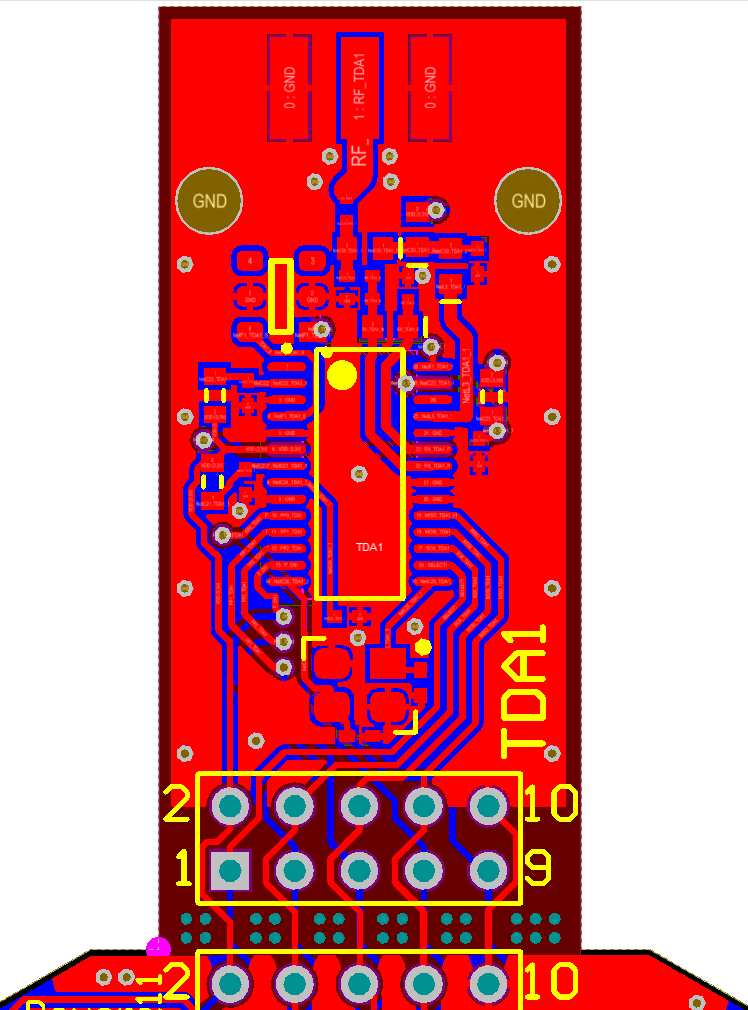
\includegraphics[trim=4.3cm 0cm 4.4cm 0cm, clip=true, totalheight=0.5\textheight,angle=-90]{Abbildungen/Aufnahmen/Bilder/Altium/TDA}
\caption{Layout des Transceivers mit der Sollbruchstelle, der Steckerleiste und dem Anpassnetzwerk}
\label{fig:tdalayout}
\end{figure}

 
Die Antenne wurde am oberen Ende jeder TDA5340-Teilplatine vorgesehen. Als Anschluss für die Antenne wurde hier eine Koaxialbuchse in \ac{SMA}-Ausführung verwendet, welche auf \unit[50]{$\Omega$} angepasst ist. Durch den Koaxialsteckverbinder konnte sichergestellt werden, dass alle notwendigen Frequenzen auch korrekt und ungedämpft passieren können. 
Das Anpassnetzwerk zwischen dem  integrierten Transceiver und der verwendeten \ac{SMA}-Buchse diente der Leistungsanpassung zwischen den Pins des TDA5340 und der \unit[50]{$\Omega$}-Koaxialbuchse. Der Aufbau des Anpassnetzwerkes basiert auf einem von Stefan Erhard erstellten Schaltplan für eine Aufsteckplatine für das Evaluationsboard \enquote{XMC 2Go} von Infineon. Durch die Verwendung von hoch abgestimmten Spulen und Kondensatoren mit Toleranzen von nur \unit[±0,05]{pF} bei einem Nennwert von \unit[2,5]{pF} wurde die korrekte Anpassung sichergestellt. 
 


 
 
 
 
Zur Verbesserung der Hochfrequenzeigenschaften wurden die Freiräume zwischen den Leiterbahnen mit einer Kupferfläche gefüllt, die mit dem Masseanschluss verbunden war. Durch die Verwendung von Vias, vor allem im Bereich des Anpassnetzwerkes, sollte eine niederohmige Verbindung zwischen den beiden Masseflächen auf der Ober- bzw. Unterseite der Platine erreicht werden. Daneben dienten diese, auf Nullpotential liegenden Vias, jedoch vor allem der Abschirmung der Pfade für die HF-Signale gegen mögliche Einkoppelungen aus der Umgebung, welche ankommende Funksignale stören könnten.

Obwohl der TDA5340 einen eingebauten Zwischenfrequenz-Filter hat, der über eine umschaltbare Bandbreite verfügt, wurde ein externer Keramikfilter verwendet. Der TDA stellt dafür zwei Pins bereit, zwischen denen ein solcher Filter mit einer Frequenz von \unit[10,7]{MHz} angeschlossen werden kann. Ohne einen hier extern angeschlossenen Filter würde der TDA als einfacher heterodyner Mischer direkt auf die Zwischenfrequenz $f_{IF2}=\unit[274]{kHz}$ heruntermischen. Bei Verwendung eines externen Keramik oder auch eines LC-$\pi$-Filters kann das ankommende HF-Signal jedoch in zwei Stufen gefiltert werden, ehe es in das Basisband demoduliert wird, was zu einer höheren Signalqualität führt. Die Umstellung zwischen einfacher und Double Down Conversion erfolgt durch das setzen eines dafür vorgesehenen Bits \cite{TDA-DataSheet}\cite{TDA-UserManual}.

Die elektrischen Verbindungen zwischen den beiden symmetrischen Eingängen des Low Noise Amplifier und dem Anpassnetzwerk wurden mit dem \enquote{Differential Pair Routing}-Feature von Altium Designer erstellt. Durch einen im Schaltplan auf die positive und negative elektrische Leitung zwischen dem TDA5340 und dem Anpassnetzwerk angewendeten Parameter wird das Leitungspaar als differentiell markiert. Anschließend kann mit dem interaktiven \enquote{Diffential Pair Routing} einer der beiden Leitungen begonnen werden. Altium Designer wird dabei selbstständig versuchen, die zweite Leiterbahn des Paares so anzuordnen, das die beiden Leiterbahnen symmetrisch und parallel zueinander liegen, sodass Störeinflüsse möglichst gleichmäßig auf die beide Leitungen einwirken. So sollen Störungen besser toleriert und durch die Symmetrische Signalübertragung insgesamt ausgeglichen werden können \cite{High-Speed-Guide}.
Durch die Verwendung des \enquote{Diffential Pair Routing} versucht Altium Designer auch die Länge der beiden Verbindungen anzugleichen. Durch die Anpassungen der differentiellen Leiterbahnen wird eine korrekte Übertragung durch gleiche Signallaufzeiten sichergestellt. Da diese Leitungen hochfrequente Signale führen, ist eine genaue Anpassung notwendig.




Um Einkopplungen auf die Pfade für hochfrequente Signale zu vermeiden, wurde das für den Transceiver benötigte Quarz möglichst weit vom Sende- bzw. von den Empfangsanschlüssen des TDA angeordnet. Aus diesem Grund wurde der für den Oszillator benötigte Quarz mit einer Frequenz $f_{Crystal}=\unit[21,948717]{MHz}$ zwischen dem \ac{IC} und der vorgesehenen Stiftleiste platziert.  Die Frequenz des benötigten Quarzes ergibt sich aus dem  Zusammenhang
\begin{equation}\label{eq:fsys}
f_{Crystal} = f_{IF2} \cdot 80 = \frac{f_{IF1}}{39} \cdot 80  = \frac{\unit[10,7]{MHz}}{39} \cdot 80 = \unit[21,948717]{MHz}
\end{equation}
wobei die Zwischenfrequenz der ersten Stufe ($f_{IF1}$) durch die internen funktionalen Blöcke des TDA und den Keramikfilter vorgegeben ist. Die weiteren Faktoren ergeben sich aus dem Aufbau des Empfängers und werden von Infineon bereitgestellt \cite{TDA-UserManual}.


\subsection{XMC4500}
\begin{figure}[h]
	\centering
	\includegraphics[trim=16cm 8cm 16cm 26cm, clip=true,width=0.7\linewidth]{"Quellen/New Infineon Controller Family/XMC4500_LQFP-100_LQFP-144_LFBGA-144"}
	\caption{Der XMC4500 Mikrocontroller von Infineon im LQFP-Gehäuse mit 144 Pins \cite{Bauer2012New-Infineon-32}}
	\label{fig:xmc4500}
\end{figure}
Die Hauptsteuerung der Basisstation übernimmt ein Mikrocontroller der Bauart XMC4500, welcher aus der Mikrocontroller-Familie XMC4000 von Infineon stammt. Diese Baureihe stellt energieeffiziente \acp{IC} bereit, welche für industrielle Steuerungen und \enquote{Sense \& Control} optimiert sind. 
Der XMC4500 basiert auf einem  Cortex\textsuperscript{TM}-M4 Kern des britischen Herstellers ARM. Daneben arbeitet der Mikrocontroller mit der von Infineon selbst entwickelte Entwicklungsumgebung DAVE zusammen.
Im speziellen Anwendungsfall kommt die Variante des XMC mit 144 Pins und einem Flash-Speicher von 1024 Kilobit zum Einsatz. Der Chip ist dabei in einem \ac{LQFP}-Gehäuse verbaut. Durch die Wahl diese Gehäuses konnte die elektrische Verbindung mit der Platine relativ leicht durch löten erreicht werden. Im Gegensatz zum ebenfalls erhältlichen \ac{BGA}-Gehäuse des XMC sind in diesem alle Kontakte direkt erreichbar und können leicht verlötet werden. Da beim \ac{BGA}-Gehäuse die Anschlüsse auch in der Mitte unter dem Gehäuse sind, wäre hier ein Layout komplizierter und würde möglicherweise einen genaueren und somit teureren Prozess für die Herstellung der Platine fordern. Ein händisches Nachlöten von Kontakten oder Prüfen der Lötverbindung wäre ebenfalls nicht möglich.



%PP2 an INterrupeingang
Bei der Auswahl von Pins des XMC zur Verbindung mit den Transceivern wurde vor allem auf die Auswahl für die PP2 Pins geachtet. Um eine spätere Interruptsteuerung möglich zu machen wurden hierfür nur solche Eingänge des Mikrocontroller gewählt, die im Datenblatt mit der Möglichkeit zum Erkennen von Interrupts gekennzeichnet waren. Die Zuordnung der Transceiverausgänge an die Pins des Mikrocontroller sind in \mbox{Abbildung \ref{fig:schemXMC}} erkennbar.

Zur Verteilung der entstehenden Abwärme wurde auch in diesem Bereich der Platine  frei gebliebene Abschnitte zwischen den Leiterbahnen mit geerdeten Kupferflächen gefüllt. Durch teilweise auch mehrfache Durchkontaktierungen wurde sowohl eine saubere Kontaktierung der Flächen durchgeführt, um Flächen schwimmenden Potentials zu vermeiden. Durch die Vias wurde aber auch die thermische Leitfähigkeit zwischen den beiden Kupferlagen erhöht und somit die Abgabe entstehender Wärme von den Bauteilen verbessert. Beim verwendeten \ac{LQFP}-Gehäuse des XMC4500 liegt die Rückseite des Halbleiters offen und ist nicht im Gehäuse verschlossen. Im Bereich unter der offenliegenden Rückseite des Chips ist deswegen zur Wärmeableitung ein Feld von 6x6 Vias vorgesehen. Dieser Aufbau dient dazu die Temperatur des Chips (junction temperature) auf den maximal erlaubten Wert $T_J = \unit[150]{^\circ C}$ zu beschränken.%Rechnung mit Therm wiederst. ??

\begin{figure}[h]
	\centering
	\includegraphics[width=\linewidth,page=5]{"../../Altium/mobile Basisstation/Project Outputs for mobile Basisstation/Basisstation Schematics"}
	\caption{Schaltplan des XMC4500 Mikrocontrollers}
	\label{fig:schemXMC}
\end{figure}


%Quarz (dämpfungswiderstand)
%Für mögliche spätere Anwendungsfälle wurde außerdem ein Quarz für die Realtime-Clock des XMC4500 vorgesehen

%Reset taster
%LEDs
Um die Ausgabe von aktuellen Systemzuständen zu ermöglichen wurden sieben Status-LEDs an freien Ausgänge des XMC4500  angeschlossen. Diese ermöglichten in active-low Ansteuerung eine Anzeige verschiedener im Mikrocontroller ablaufender Prozesse. Für vier der verwendeten Leuchtdioden wurde grün als Farbe gewählt, für die drei weiteren rot. Zur Vereinfachung eines Resets der Hardware wurde ein entsprechender Taster vorgesehen, mit dem der entsprechenden  $\overline{\text{PORST}}$-Pin des Mikrocontroller auf das 0V Potential gezogen wird und somit die Hardware zurückgesetzt wird.
Die Programmierung des Mikrocontrollers erfolgt über das \ac{JTAG}-Interface über welches auch das debuggen möglich ist. Der XMC4500 stellt dafür ein \ac{JTAG}-Modul bereit, welches mit den in IEEE 1149.1 festgelegten Standarts übereinstimmt. Verwendet wird hierfür die achtpolige Variante des Debug-Steckers, bei dem der Platine vom \ac{JTAG}-Adapter Versorgungsspannung und Masse sowie Signale für Reset, Systemtakt und die Steuerleitung übergeben wird.  %enquote xmc DAtenblatt , nur zwei angeschlossen?

%Abblockkondensatoren

Für die Kommunikation des Mikrocontroller mit einem Computer wird die im XMC  bereitgestellte Peripherie genutzt. Zur Verbindung mit einem anderen Gerät wurde deshalb eine kombinierte Micro-USB-Buchse verwendet welche sowohl für Typ A oder Typ B Stecker geeignet ist.
Um sowohl den Mikrocontroller als auch einen an die Basisstation angeschlossenen Computer gegen Fehlerströme über die USB-Leitung zu schützen wurden die Datenleitungen mit so genannten \ac{TVS}-Dioden , welche gegen Masse geklemmt sind, geschützt. Sowohl positive als auch negative Spannungsspitzen werden dadurch gegen Masse kurzgeschlossen, was zum Schutz des XMC bzw. des angeschlossenen Computer dient. Um eine Verpolung bei Stromversorgung über die USB-Buchse, und somit eine Zerstörung, zu vermeiden wurde eine Schottky-Diode im Strompfad zum Spannungsregler vorgesehen. Diese soll einen Stromfluss im Verpolungsfall unterbinden. Für den Fall das zeitgleich ein Netzteil sowie eine stromversorgende USB-Verbindung angeschlossen ist, dienen die Schottky-Dioden ebenfalls dem Schutz der Bauteile. Da der Mikrocontroller für die Kommunikation über das USB-Interface die aktuelle Busspannung auf der USB-Leitung benötigt, muss der extra dafür vorgesehene Pin des XMC direkt und ohne schützende Schottky-Diode mit der 5V Leitung der USB-Buchse verbunden werden. 


\subsection{Ethernet}
Die Ethernetschnittstelle der Basisstation basiert auf dem  Relax Kit von Infineon. Genau wie im Evaluations Board des Herstellers Infineon wurde der Ethernet-Controller KSZ8031RNL von Mircel Inc. verwendet. Dieser stellt alle wichtigen Peripherien selbst zur Verfügung und muss somit nur noch durch ein Quarz und diverse Kapazitäten und Induktivitäten an den Versorgungsleitungen ergänzt werden. Da die im Controller verbaute Stufe zur Interruptgenerierung nur über einen schwachen Pull-Up Widerstand verfügt, musste ein externer Widerstand von \unit[1]{k$\Omega$} verbaut werden. Am Reset-Eingang wurde ebenfalls ein Pull-Up Widerstand verbaut. Dieser wurde um zwei Dioden sowie einen Kondensator zu der im Datenblatt empfohlenen Verschaltung erweitert. So kann sichergestellt werden, das sowohl beim Anlegen einer Spannung an das Gesamtsystem als auch bei einem Reset des Ethernetbausteins durch den steuernden Mikrocontroller alle Spannungen im sicheren Bereich liegen und die Funktion gewähleistet ist. Die dreizehn zum XMC4500 notwendigen Verbindungen wurden zur besseren Übersicht im Schaltplan in einem Signal-Kabelbaum zusammengefasst. Wegen der Gefahr von Rissen in Lötstellen durch die Platinenbelastung beim Ein- und Ausstecken wurde im Bereich um den Netzwerkstecker die Anordnung von Bauteilen vermieden. 
Da der KSZ8031RNL  nicht lieferbar war und die anfallende Datenmenge nur von geringem Umfang ist, wurde der Controller und die entsprechende Netzwerkbuchse von Würth Electronics zunächst nicht bestückt. Somit wurde eine Verwendung des Ethernet-Controllers auch in der Software des XMC-Mikrocontroller nicht umgesetzt. Da jedoch ein entsprechendes Softwareprojekt für das Relax Kit von Infineon zur Verfügung gestellt  wird, wäre eine Netzwerkkommunikation vermutlich mit wenigen Anpassungen schnell umzusetzen \cite{DAVE-3-Example-}. 








\subsection{Spannungsversorgung}
Die Bereitstellung der notwendigen Spannung sollte wahlweise über den zur Datenerfassung angeschlossenen Computer oder über ein externes Netzteil erfolgen. Zum Anschluss eines externen Netzteils wurden Lötanschlüsse für eine Steckerleiste im Rastermaß \unit[2,54]{mm} vorgesehen. Genau wie bei der Stromversorgung über die USB-Buchse wurde auch hier eine Schottky-Diode zum Verpolungsschutz der Schaltung integriert. Ausgelegt ist die Basisstation für ein Gleichspannungsnetzteil mit \unit[5]{V} Ausgangsspannung, durch den Aufbau mit den beiden verwendeten Schottky-Dioden und die mögliche Eingangsspannung des nachfolgenden Reglers wäre jedoch auch eine angeschlossene \unit[6]{V}-Stromquelle (bei vernachlässigtem Spannungsabfall an der Diode) unproblematisch.
Wegen der bereits erwähnten notwenigen Versorungspannung von \unit[3,3]{V} für den XMC4500 und die Transceiver wurde diese mit einem \ac{LDO}-Regler aus externen angeschlossenen Spannungsversorgung generiert. Dieser verwendete Spannungsregler der Bauart MCP1826S von Microchip Technology Inc. sollte die Eingangspannung auf das gewünschte Niveau herunter regeln.
Als Gehäusetyp wurde das dreibeinige \ac{SOT}-Package gewählt, da keine Variante des \ac{LDO} mit einstellbarer Ausgangsspannung und somit keine Variante des \acp{IC} mit mehr Anschlusspins benötigt wurde. Statt des \ac{LDO} von Microchip war zunächst ein gleichwertiger Spannungsregler von Infineon, der IFX1117MEV33, vorgesehen. Die beiden \acp{LDO} unterscheiden sich in der elektrischen Belegung der Kühlfahne des \ac{SOT}-223: beim Spannungsregler von Infineon ist diese mit dem \unit[3,3]{V} Output kontaktiert, beim verwendeten \ac{LDO} mit Ground. Da es sich bei dem Spannungsregler um ein \ac{SMD}-Bauteil handelt, ist die Verwendung von Kühlkörpern schwer möglich. Die Abführung der im Spannungsregler erzeugten Verlustwärme erfolgt deshalb üblicherweise über das Anlöten der Kühlfahne an eine genügend große Kupferfläche, die als Wärmesenke dient. So wird die erzeugte Wärme gespreizt und kann gut an die Umgebung abgegeben werden. Bei Verwendung des zuerst eingeplanten IFX1117MEV33 wäre somit eine Kupferfläche auf \unit[3,3]{V} Potential zum Kühlen notwendig, welche elektrisch isoliert sein müsste. Wegen des Platzbedarfs durch den XMC4500 und andere Bauteile wäre somit nur eine Kupferfläche mit Abmessungen von etwa \unit[15]{mm} auf \unit[16]{mm} möglich, da die elektrischen Verbindungen bestehender Bauteile des Bereiches nicht unterbrochen werden sollten. Durch die Verwendung des entsprechenden Bauteils von Microchip konnte auf eine abgetrennte Kupferinsel verzichtet werden und somit die bereits erwähnte \acs{GND}-Kupferfläche um den Mikrocontroller als gemeinsame Masse- und Kühlfäche verwendet werden.
Wegen der vorderseitigen Bauteilbestückung war die verfügbare Kupferfläche auf der Platinenrückseite  größer. Um dies beim Ableiten der Wärme vom Bauteil zu nutzen, wurden vor allem im Bereich um die Kühlfinne des \ac{SOT}-223 Gehäuses Durchkontaktierungen angebracht. Diese parallelen \enquote{Thermal Vias} konnten als Wärmepfad zur unteren Kupferfläche dienen. Außerdem wurde der \ac{JTAG}-Stecker des XMC absichtlich im Bereich neben dem Spannungsregler angebracht. Durch die große Oberfläche stellt auch dieser eine gute Wärmesenke dar. %sicher?
% Rechnung Thermischer widerstand

\section{Generierte Dokumente}
Altium Designer kann aus den erstellten \ac{PCB}-Daten die für die weitere Verarbeitung benötigten Dateien generieren. Im dazu vorgesehene Output-Job-Manager können entsprechende Outputs gewählt werden und einem Output-Container zugeordnet werden. Dies ist vor allem zum Erstellen gewünschter Dateistrukturen bei größeren Projekten notwendig um diese übersichtlich zu halten. Im der vorliegenden Arbeit wurde dies jedoch nur bedingt benötigt.
Für die Bestückung der Basisstation wurde zunächst eine \enquote{Bill of materials}, also eine Materialliste, exportiert mit deren Hilfe die entsprechenden Bestellnummern des Lieferanten Digi-Key herausgesucht und sortiert werden konnten. Mithilfe der ebenfalls generierten \enquote{Assembly Drawings} war die Ausgabe aller Bauteile und deren Platzierung auf der Platine möglich. Ebenfalls wurden in diesem Menü die strukturierten Schaltpläne ausgegeben.

Zur dreidimensionalen Visualisierung wurde die fertige Platine mit den in den Footprints enthaltenen Bauteilabmessungen und Höhen als 3D-Modell im \ac{STEP}-Format ausgegeben. Mithilfe des \ac{CAD}-Programms \enquote{SolidWorks} wurde daraus ein Gehäuse mit Deckel für die Basisstation erstellt. Diese wurde anschließend mit einem 3D-Drucker ausgedruckt und dient dazu, die Platine zu schützen.

Die Fertigung der Platine durch den Hersteller erfolgte durch so genante Gerber Daten, die ebenfals aus dem Output-Job-Manager generiert wurden. Dabei wird für jedes Layer des \ac{PCB}-Editors eine Gerberdatei erstellt, in der die Geometrie der entsprechenden Lage angegeben ist. Jede Lage entspricht in der Herstellung dabei einem Fertigungsschritt. Um Bohrungen in der Platine zu setzen, werden zusätzliche \enquote{NC Drill-Files} also Daten für die \ac{NC} der automatischen Maschinen zum setzen von Bohrungen. Diese enthalten den Bohrdurchmesser, die Art der Bohrung sowie den Ort auf der Platine und müssen zusätzlich aus Altium Designer exportiert werden. Solche Bohrungen sind sowohl für Vias, als auch für Befestigungsbohrungen notwendig.


\section{Bestückung}
Die gefertigte Platine wurde vor der Programmierung mit den notwendigen Bauteilen bestückt. Dabei wurde zuerst der XMC4500 mit einer Bestückungsmaschine auf dem vorgesehenen Footprint der Platine verlötet. Im folgenden wurden alle weiteren Bauteile sowie die sechs Transceiver mit Lötpaste auf der Platine befestigt und anschließend durch Erhitzen der Platine auf der Heizplatte verlötet. Das kontaktieren durch die Heizplatte wurde in mehreren Schritten durchgeführt. Dabei wurden zunächst Bauteile einer guten Toleranz hoher Temperaturen wie Stecker und Widerstände bestückt. Temperaturanfällige Bauteile wie Leuchtdioden und integrierte Schaltkreise wurden nach Möglichkeit zu einem späterem Zeitpunkt befestigt. Wie bereits erwähnt wurde der Ethernet-Controller nicht bestückt.

